\subsection*{19.1}
International trade has no ambiguity, it is good and has the ability to make everyone better off.\\
Free trade means voluntary exchange between two countries.\\
The gain from free trade is always greater than the loss.\\
Closing borders gives market power to the producers and they can charge higher prices.\\
The difference between the price of an "evil" product and its counterpart shows how much society values the cause of the counterpart.
\par
David Ricardo created a model that shows how two countries can benefit from trade.\\
Imagine two countries, and two goods.\\
Trade is not based on absolute advantage, but comparative advantage.\\
A country that doesn't trade is called autarky.
\begin{figure}[H]
    \centering
    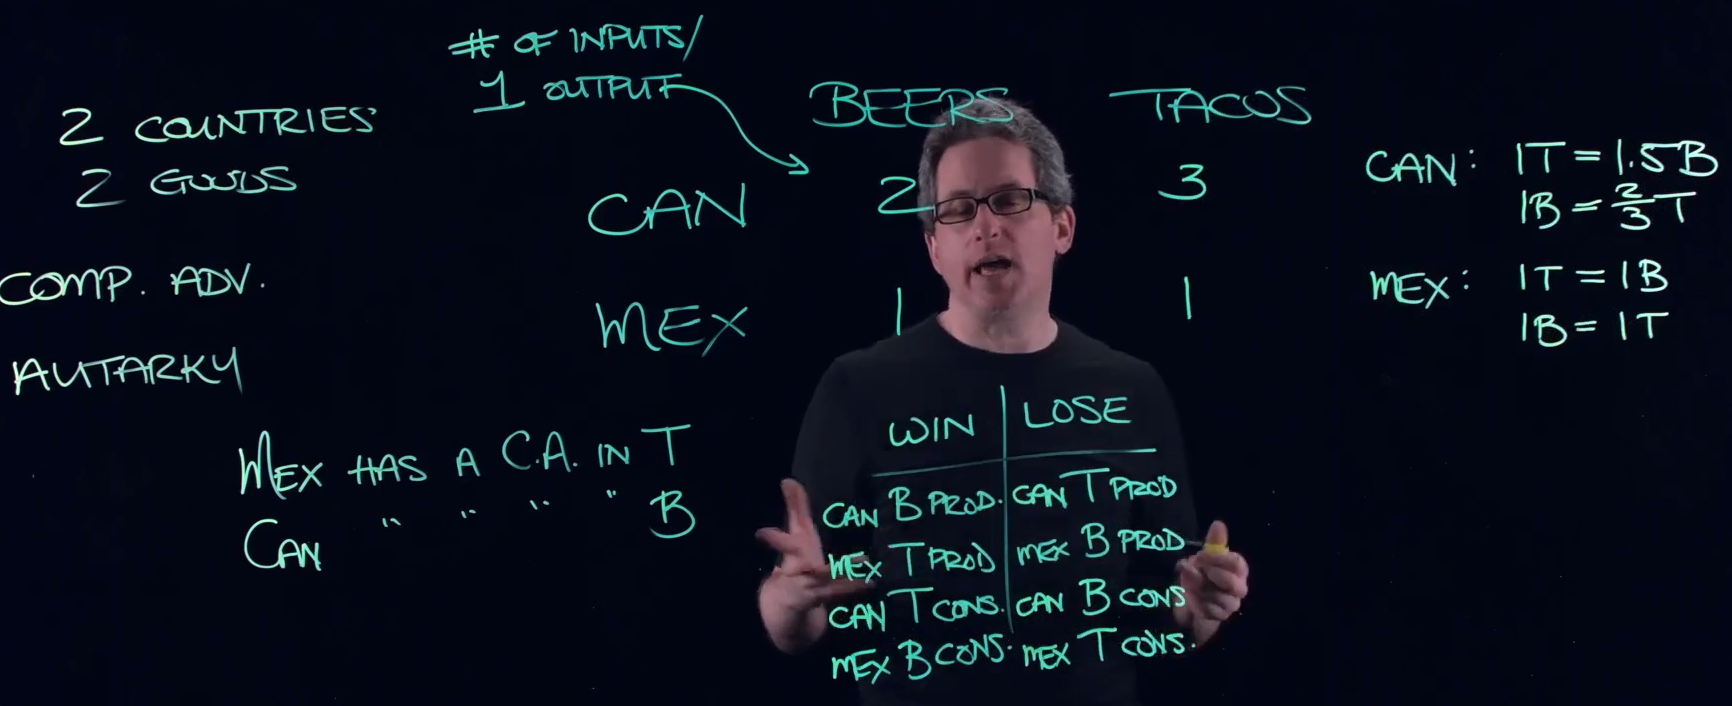
\includegraphics[width=0.5\textwidth]{Chapter19/ComparativeAdvantage.png}
    \caption{Comparative Advantage}
    \label{fig:comparativeadvantage}
\end{figure}
In this example, Mexico should export tacos, and Canada should export beer.\\
Open to trade means open to immigration and emigration too.
\par
Outside of autarky, the price of a good falls between the two countries.
\begin{figure}[H]
    \centering
    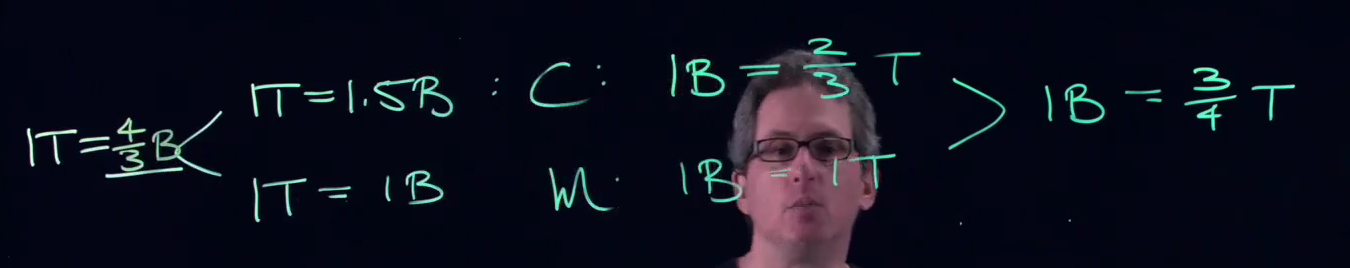
\includegraphics[width=0.5\textwidth]{Chapter19/GlobalPrice.png}
    \caption{Global Price}
    \label{fig:globalprice}
\end{figure}
\par
We can also look at the production possibility frontier with the budget constraint and indifference curve for the entire country in autarky.\\
The excess or shortage of a leads to export/imports.\\
This won't work in the real world because the declining industry will protest.
\begin{figure}
    \centering
    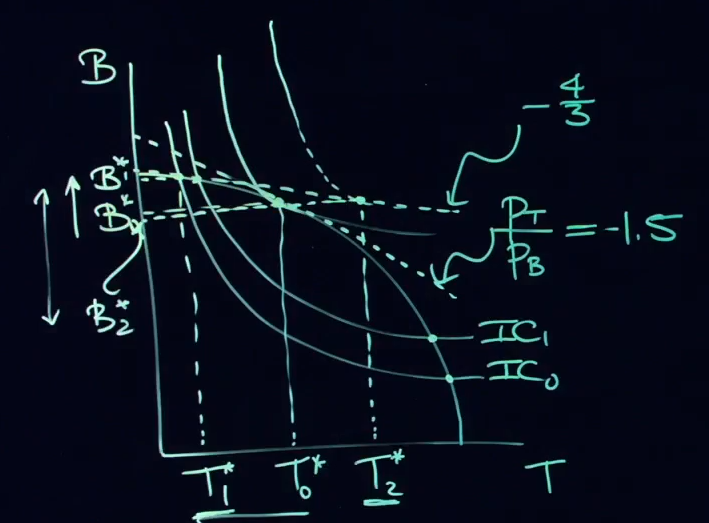
\includegraphics[width=0.5\textwidth]{Chapter19/PPF.png}
    \caption{Production Possibility Frontier}
    \label{fig:ppf}
\end{figure}
\par
Some countries have a comparative advantage due to natural resources, learning by doing, cultural affinity and proximity.\\
Comparative advantages can change over time.